\begin{center}
\begin{minipage}{0.49\textwidth}
\begin{center}
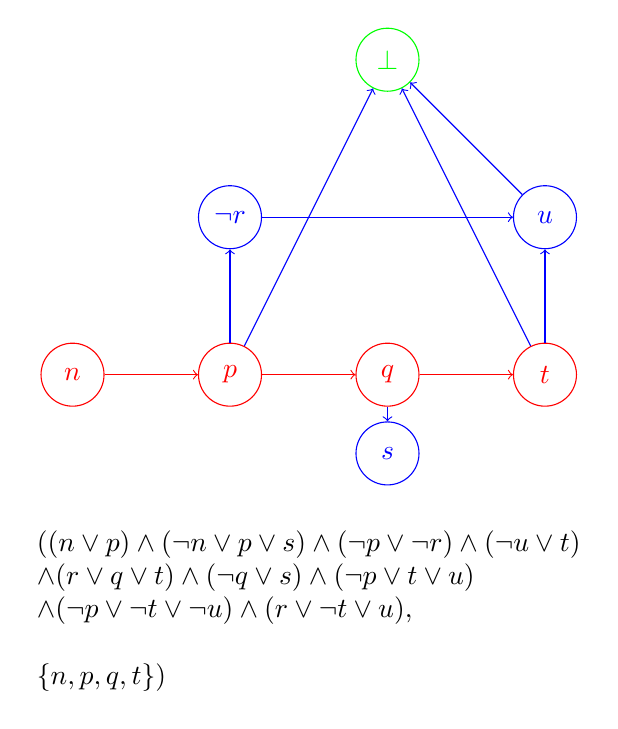
\begin{tikzpicture}
\node (n) [draw, circle, red, align=center, minimum size=0.8cm] at (0,0) {$n$};
\node (p) [draw, circle, red, align=center, minimum size=0.8cm] at (2,0) {$p$};
\node (q) [draw, circle, red, align=center, minimum size=0.8cm] at (4,0) {$q$};
\node (t) [draw, circle, red, align=center, minimum size=0.8cm] at (6,0) {$t$};
\node (s) [draw, circle, blue, align=center, minimum size=0.8cm] at (4,-1) {$s$};
\node (r) [draw, circle, blue, align=center, minimum size=0.8cm] at (2,2) {$\lnot r$};
\node (u) [draw, circle, blue, align=center, minimum size=0.8cm] at (6,2) {$u$};
\node (conflict) [draw, circle, green, align=center, minimum size=0.8cm] at (4,4) {$\bot$};

\draw [->, red] (n) -- (p);
\draw [->, red] (p) -- (q);
\draw [->, red] (q) -- (t);

\draw [->, blue] (p) -- (r);
\draw [->, blue] (p) -- (conflict);
\draw [->, blue] (q) -- (s);
\draw [->, blue] (t) -- (u);
\draw [->, blue] (t) -- (conflict);
\draw [->, blue] (r) -- (u);
\draw [->, blue] (u) -- (conflict);

\node (formula1) [align=left] at (3, -3) {($(n\lor p) \land(\lnot n\lor p\lor s) \land (\lnot p \lor \lnot r) \land (\lnot u \lor t)$ \\ $ \land (r\lor q \lor t) \land(\lnot q\lor s) \land (\lnot p\lor t \lor u)$ \\ $\land (\lnot p\lor \lnot t\lor \lnot u) \land (r\lor \lnot t\lor u)$, \\
\\
$\{n, p, q, t\}$)};
\end{tikzpicture}
\end{center}
\end{minipage}
\begin{minipage}{0.49\textwidth}
\begin{center}
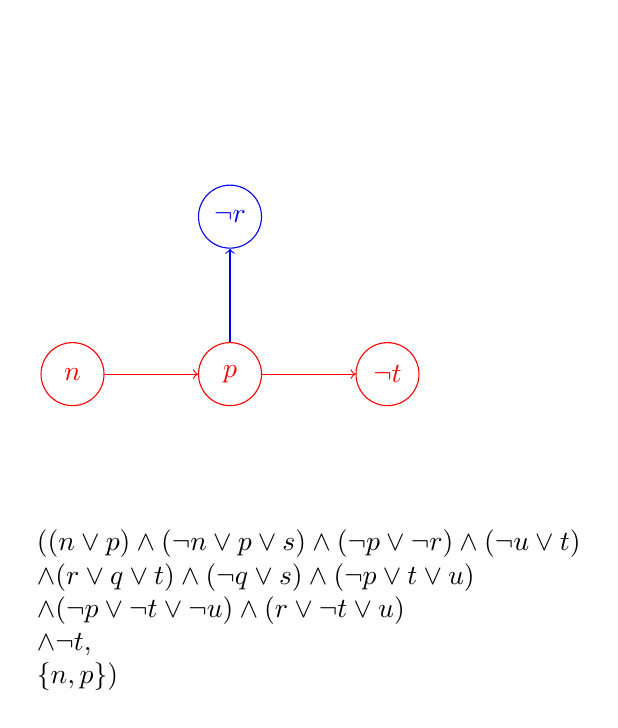
\begin{tikzpicture}
\node (n) [draw, circle, red, align=center, minimum size=0.8cm] at (0,0) {$n$};
\node (p) [draw, circle, red, align=center, minimum size=0.8cm] at (2,0) {$p$};
\node (t) [draw, circle, red, align=center, minimum size=0.8cm] at (4,0) {$\lnot t$};
\node (r) [draw, circle, blue, align=center, minimum size=0.8cm] at (2,2) {$\lnot r$};
\node (x) [minimum size=0.8cm] at (4,4) {};

\draw [->, red] (n) -- (p);
\draw [->, red] (p) -- (t);

\draw [->, blue] (p) -- (r);

\node (formula1) [align=left] at (3, -3) {($(n\lor p) \land(\lnot n\lor p\lor s) \land (\lnot p \lor \lnot r) \land (\lnot u \lor t)$ \\ $ \land (r\lor q \lor t) \land(\lnot q\lor s) \land (\lnot p\lor t \lor u)$ \\ $\land (\lnot p\lor \lnot t\lor \lnot u) \land (r\lor \lnot t\lor u)$ \\
$\boldsymbol{\land \lnot t}$, \\
$\{n, p\}$)};
\end{tikzpicture}
\end{center}
\end{minipage}
\captionof{figure}{Example implication graph before and after back-jumping.}
\end{center}
